\section[Introduction]{Introduction\protect\footnote{This section is based on work submited to the American Institude of Physics, Physics of Fluids journal.
                        It is reproduced from submission number \#POF25-AR-DSFD2024-03180, with the permission of AIP Publishing.}}

Bicontinuous interfacially jammed emulsion gels (bijels) are a class of particle-stabilized emulsions composed of two interpenetrating, tortuous domains separated by a jammed layer of colloidal particles 
at the interface \cite{stratford_colloidal_2005, herzig_bicontinuous_2007, tavacoli_novel_2011}. Bijels form when neutrally wetting particles are suspended in a binary fluid mixture undergoing spinodal 
decomposition. As the domains coarsen, the particles irreversibly adsorb onto the interface and eventually jam when the available interfacial area matches the total cross-sectional area of the particles. 
This jamming arrests coarsening and locks in the bicontinuous morphology. Owing to their tunable structure, bijels have been proposed as templates for porous materials with potential applications in 
energy storage, filtration, and catalysis \cite{yabuno_preparation_2020, samdani_bicontinuous_2017, cha_bicontinuous_2019, garcia_scalable_2019, santiago_cordoba_aerobijels_2020}.

Stimuli-responsive emulsions have gained increasing attention for use in enhanced oil recovery, porous material templating, in-situ separation processes, and drug delivery systems 
\cite{tang_stimuli-responsive_2016, bago_rodriguez_capsules_2019, nakayama_stimuli-responsive_2018}. These applications exploit the ability of emulsions to undergo structural transformations in response 
to external stimuli, leading to changes in permeability, surface area, and morphology. We recently demonstrated that bijels stabilized by magnetically responsive ellipsoidal particles exhibit anisotropic 
structures when subjected to external magnetic fields \cite{karthikeyan_formation_2024}. Characterization of the domain size and tortuosity revealed significant field-induced anisotropy, indicating that 
magnetic fields can modulate the structural features of the bijel template.

While the characteristic domain size \(L\), often derived from the structure factor as \(L = \frac{2\pi}{q^*}\), is commonly used to quantify emulsion coarsening, this scalar measure alone cannot capture the 
geometrical complexity or topological features of the microstructure \cite{kendon_inertial_2001}. Prior studies have highlighted the relevance of local topology and morphology in determining the performance of 
porous materials \cite{liu_influence_2021, xiong_porosity_2024, shojaei_minimal_2022}. For example, mechanical properties and cell proliferation in bone scaffolds have been shown to depend on local topological 
characteristics \cite{xiong_porosity_2024}, and optimized gas transport in diffusion membranes has been achieved by tuning microstructural connectivity and wettability \cite{shojaei_minimal_2022}. 

Within the bijel literature, Reeves et al.~investigated how particle size and quench rate affect bijel formation, showing that nanoparticles enable bijel synthesis under conditions where microparticles fail 
\cite{reeves_particle-size_2015}. In a follow-up study, they quantified interfacial curvature to reveal that smaller particles and faster quenches result in more negative Gaussian curvature, enhancing the 
hyperbolic character of the structure \cite{reeves_quantitative_2016}. While the curvature is an microstructural metric, information about the topology of the interface provides details about the 
connectivity of the surface. \cite{mendoza_evolution_2006,chan_channel_2012} Thornton and co-workers use a topological approach to characterize the channel sizes of co-continuous porous materials, 
by measuring the topological characteristics of a surface contour as a function of distance from the interface. \cite{chan_channel_2012} McDevitt et al.~further characterized bijels by computing the pore 
size distribution using a medial ball algorithm, showing that bijels exhibit narrower and more uniform pore sizes than other emulsion-derived materials due to their co-continuous morphology 
\cite{mcdevitt_microstructural_2019}. The domain anisotropy characterized in Karthikeyan and Schiller was driven through orientations of particles on the interface towards the magnetic field, causing directional
cessation of coarsening, 'locking in' the anisotropic microstructure. Using the radial distribution function, peak shifts were characterized which indicated more ordered arrangements of particles
on the interface. However the impact and degree of greater interfacial order has not been quantified, nor has it been linked to the microstructure of the bijel. 

In this study, we conduct a detailed structural investigation of bijels stabilized by magnetic ellipsoidal particles. Leveraging data obtained from hybrid Lattice Boltzmann-Molecular Dynamics simulations of a 
binary fluid containing suspended magnetic ellipsoids, we examine the bond orientational order of the interfacial particle layer throughout the coarsening process and in the jammed state. Although indications 
of local hexagonal ordering emerge at the interface, the overall particle arrangement remains disordered due to the three-dimensional curvature of the interface. We further explore how the mean 
and Gaussian curvatures of the interface, averaged over the structure, respond to variations in applied magnetic field strength. Our findings indicate that magnetic fields may even enhance the 
inherent hyperbolic geometry of the bijel interface. Additionally, we track the topological development of the bijel network during coarsening by quantifying the number of time evolution of the number of channels
over time. This topological analysis enables the calculation of channel size distributions, which we find to align well with other conventional measures of domain size. Overall, our findings offer a comprehensive 
understanding of the structural characteristics of bijels formed with magnetically responsive ellipsoids and provide a foundation for design strategies in applications requiring tailored porous material 
microstructures.

\section{Results}
% \section[Results]{Results\protect\footnote{This section is based on work submited to the American Institude of Physics, Physics of Fluids journal.
%                     It is reproduced from submission number \#POF25-AR-DSFD2024-03180, with the permission of AIP Publishing.}}

During spinodal decomposition of a binary liquid containing magnetic ellipsoidal particles, the formation of a bijel is governed by the combined influence of capillary and magnetic torques acting on 
the particles. The applied magnetic field exerts a torque that tends to align the dipole moments of the particles with the field direction. Concurrently, the advancing liquid-liquid interface collects 
particles and applies a capillary torque, favoring alignment of the particles major axis with the interface to minimize interfacial energy. The competition between these torques influences the 
coarsening process and results in an anisotropic domain morphology. This anisotropy manifests as directional variations in domain size, tortuosity, and jamming time relative to the orientation of 
the magnetic field \cite{karthikeyan_formation_2024}. In the present work, we extend this analysis by examining the structural organization of the interfacial particle monolayer and the evolution 
of interfacial curvature. Additionally, we characterize the topology of the bijel through measures such as the channel size distribution, which provides further insight into the underlying coarsening 
mechanisms in magnetically influenced systems.

\begin{figure}
\centering
\includegraphics[scale = 0.4]{../figures/results/paper1_5/particle_layer.png}%
\caption{Visualizations of the order parameter $\phi$ for bijels stabilized by oblate (left), spherical (middle) and prolate (right) particles 
         after $10^5$ simulation time steps. The top row shows the structure of bijels formed in the 
         absence of a magnetic field, while the bottom row shows the structure of bijels formed at $\bar{B} = 1$. 
         The direction of the magnetic field is indicated by the arrow.
\label{fig:particle_layer}}%
\end{figure}

We simulated bijel formation following the procedure outlined in Section~\ref{section:sim_setup}, using magnetic particles of varying shape—spherical (\(\alpha = 1\)), oblate (\(\alpha = 0.5\)), 
and prolate (\(\alpha = 2.0\))—at a fixed volume fraction of \(\phi_p = 0.15\). The external magnetic field strength was varied across a range of reduced field values \(\bar{B} = [0, 0.2, 0.5, 1.0]\). 
Snapshots of the final configurations are shown in Fig.~\ref{fig:microstructure_viz}, illustrating the arrangement of particles at the liquid-liquid interface for each shape and field strength. As the 
field strength increases, we observe notable changes in the interfacial particle structure. In particular, the field induces alignment of the particle symmetry axes along the field direction, and this 
orientational ordering appears to promote enhanced local packing within the interfacial monolayer. To quantify this effect, we assess whether the magnetic field leads to increased bond orientational 
order within the particle layer, thereby linking field-induced alignment to changes in monolayer structure.

\subsection{Bond orientational order within the particle layer}

To quantitatively assess the local arrangement of particles at the interface, we compute the ensemble-averaged Steinhardt bond orientational order parameters $q_2$ and $q_6$.
\cite{steinhardt_bond-orientational_1983, lechner_accurate_2008, mickel_shortcomings_2013}. These parameters characterize the local structural ordering by projecting the orientations of neighboring particles 
onto spherical harmonics of degree \(l\), and are defined as


\begin{equation}
% q_l(i) = \left( \frac{4\pi}{2l+1} \sum_{m=-l}^{l} \left| \frac{1}{N(i)} \sum_{j=1}^{n(i)} Y_{lm}(\vec{r}_{ij}) \right|^2 \right)^{\frac{1}{2}} ,
q_l(i) = \sqrt{ \frac{4 \pi}{2l + 1} \Sigma_{m = -l}^{l} | \Sigma_{f} \frac{A(f)}{A}, Y_{lm}(\theta_f, \phi_f) |^2 }
\label{eq:steinhardt_definition}
\end{equation} 

Here $A(f)$ denotes the area of face f of the Voronoi cell around a reference particle, $A$ is the surface area of the Voronoi cell, 
$\theta_f$ and $\phi_f$ are the polar and azimuth angles of the outer normal vector connecting the reference particle to the vertex representing
an adjacent particle and $Y_{lm}$ is the spherical harmonic component. 
Neighbor lists are typically defined using a fixed cutoff radius around each particle, identifying nearby particles as neighbors. 
We calculate the python package Freud to calculate the bond order parameters and use a Voronoi cell to determine the particle neighborhood rather than the standard distance criterion 
\cite{ramasubramani_freud_2020,mickel_shortcomings_2013}. The Voronoi-based method avoids the need for a predefined cutoff and yields more robust neighbor definitions, particularly in disordered systems. 
Bond orientational order parameters have been widely employed to study structural transitions in colloidal and ceramic systems, including crystallization, nucleation, and glass formation 
\cite{vagberg_glassiness_2011, besseling_three-dimensional_2007, schall_structural_2007, ozawa_jamming_2012}. $q_6$ is most commonly used to identify crystal structures by matching the calculated
values to reference values for specific crystal structures such as fcc or hcp. However, Kapfer et al. pointed out that only using $q_6$ can result in false positives for amorphous systems. \cite{kapfer_jammed_2012}
Mickel et al. identified that $q_2$ vanishes for ordered crystal arrangements and is finite for disordered particle arrangements. \cite{mickel_shortcomings_2013} Therefore we report both to
characterize the particle layer. 

\begin{figure}
\centering
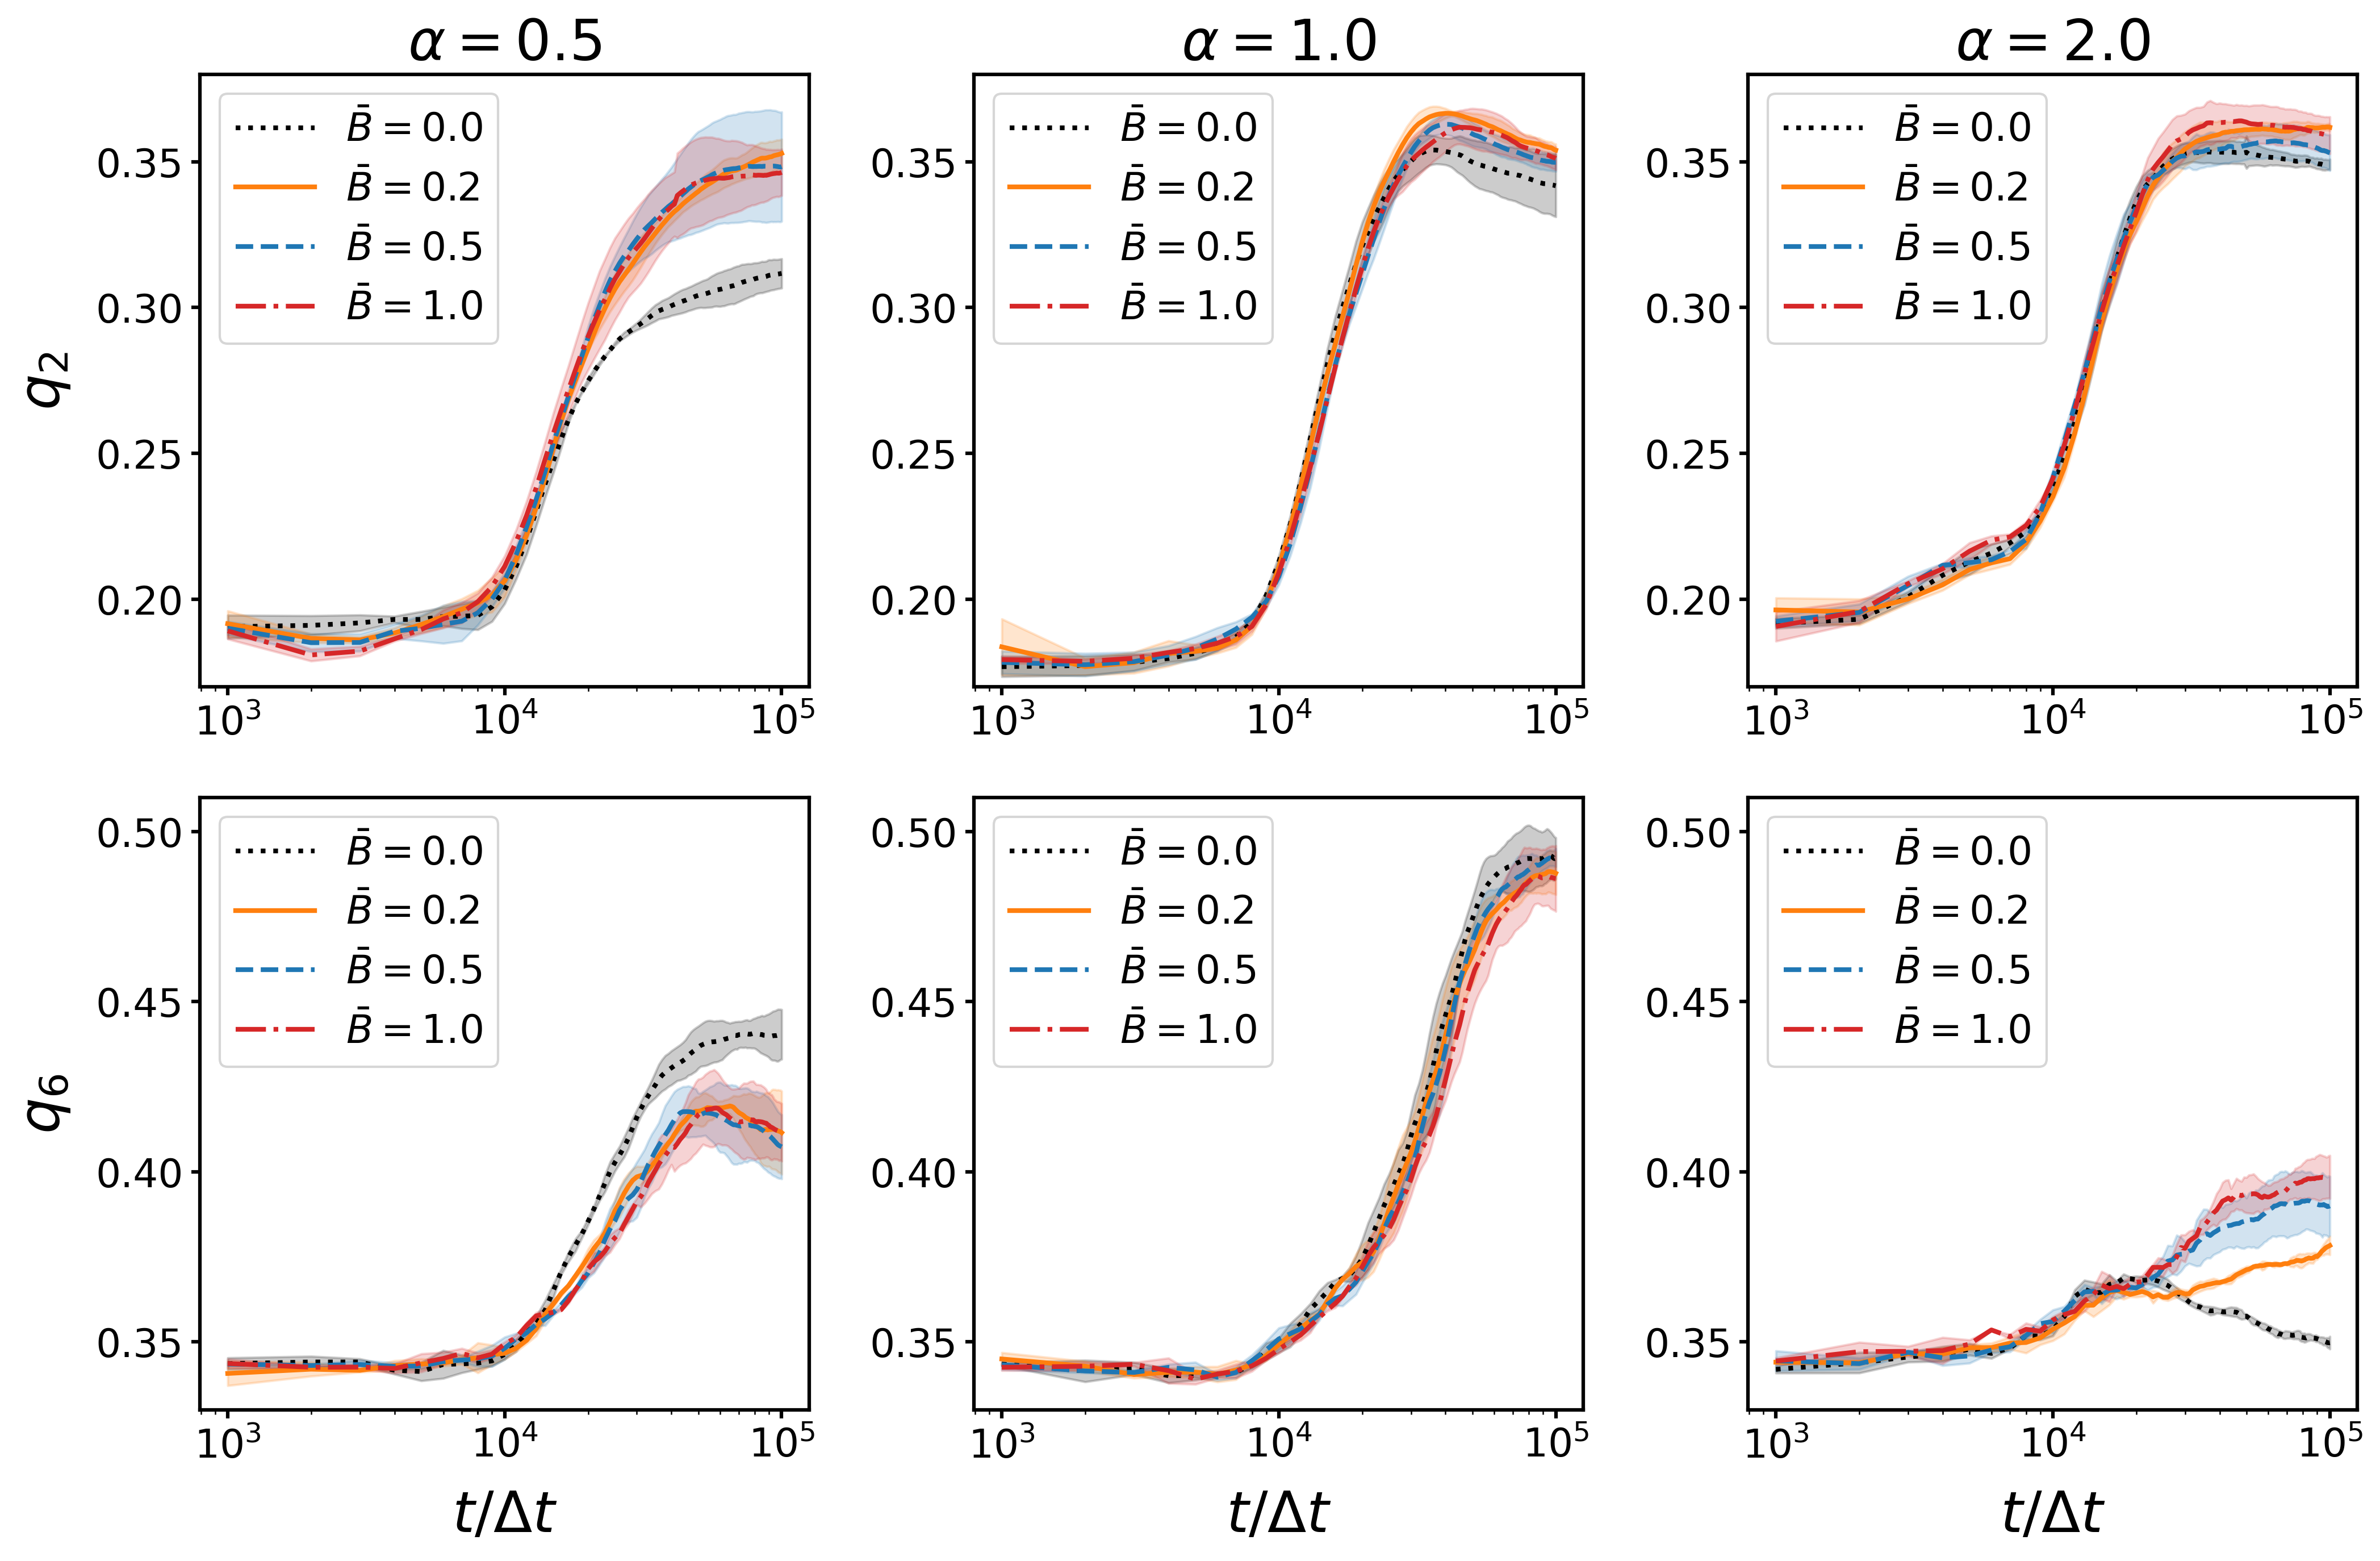
\includegraphics[scale = 0.38]{../figures/results/paper1_5/steinhardt_time.png}%
\caption{Time dependence of the Steinhardt order parameters $q_2$ and $q_4$ for different particles shapes $\alpha$ and at different magnetic field strengths $\bar{B}$. The filled bands around the lines indicate the standard deviation over three independent simulation runs.}
\label{fig:steinhardt_time}%
\end{figure}

Figure~\ref{fig:steinhardt_time} shows the time evolution of the Steinhardt order parameters \(q_2\) and \(q_6\) for all simulated magnetic field strengths and particle shapes. Both parameters begin 
to rise sharply around \(10^4\) timesteps, aligning with the onset of interfacial jamming and the deceleration of domain coarsening previously reported in \cite{karthikeyan_formation_2024}. This increase 
reflects closer packing of particles at the interface, where enhanced local density amplifies the contributions of neighboring particles to the order parameters. The growth in \(q_6\) indicates a 
rise in six-fold orientational order, as also qualitatively seen in the particle arrangements shown in Fig.~\ref{fig:particle_layer}. However, the persistence of finite \(q_2\) values suggests that the 
monolayers remain disordered. Despite visual indications of local order in the 2D interfacial projections, the three-dimensional curvature of the interface causes angular deviations between neighboring 
particle vectors \(\vec{r}_{ij}\), resulting in non-canceling contributions to the \(Y_{2m}(\vec{r}_{ij})\) terms. These results are consistent with previous findings that characterize bijels as two-dimensional 
colloidal glasses embedded within a curved, three-dimensional structure \cite{ching_bijel_2022}.

\begin{figure}
\centering
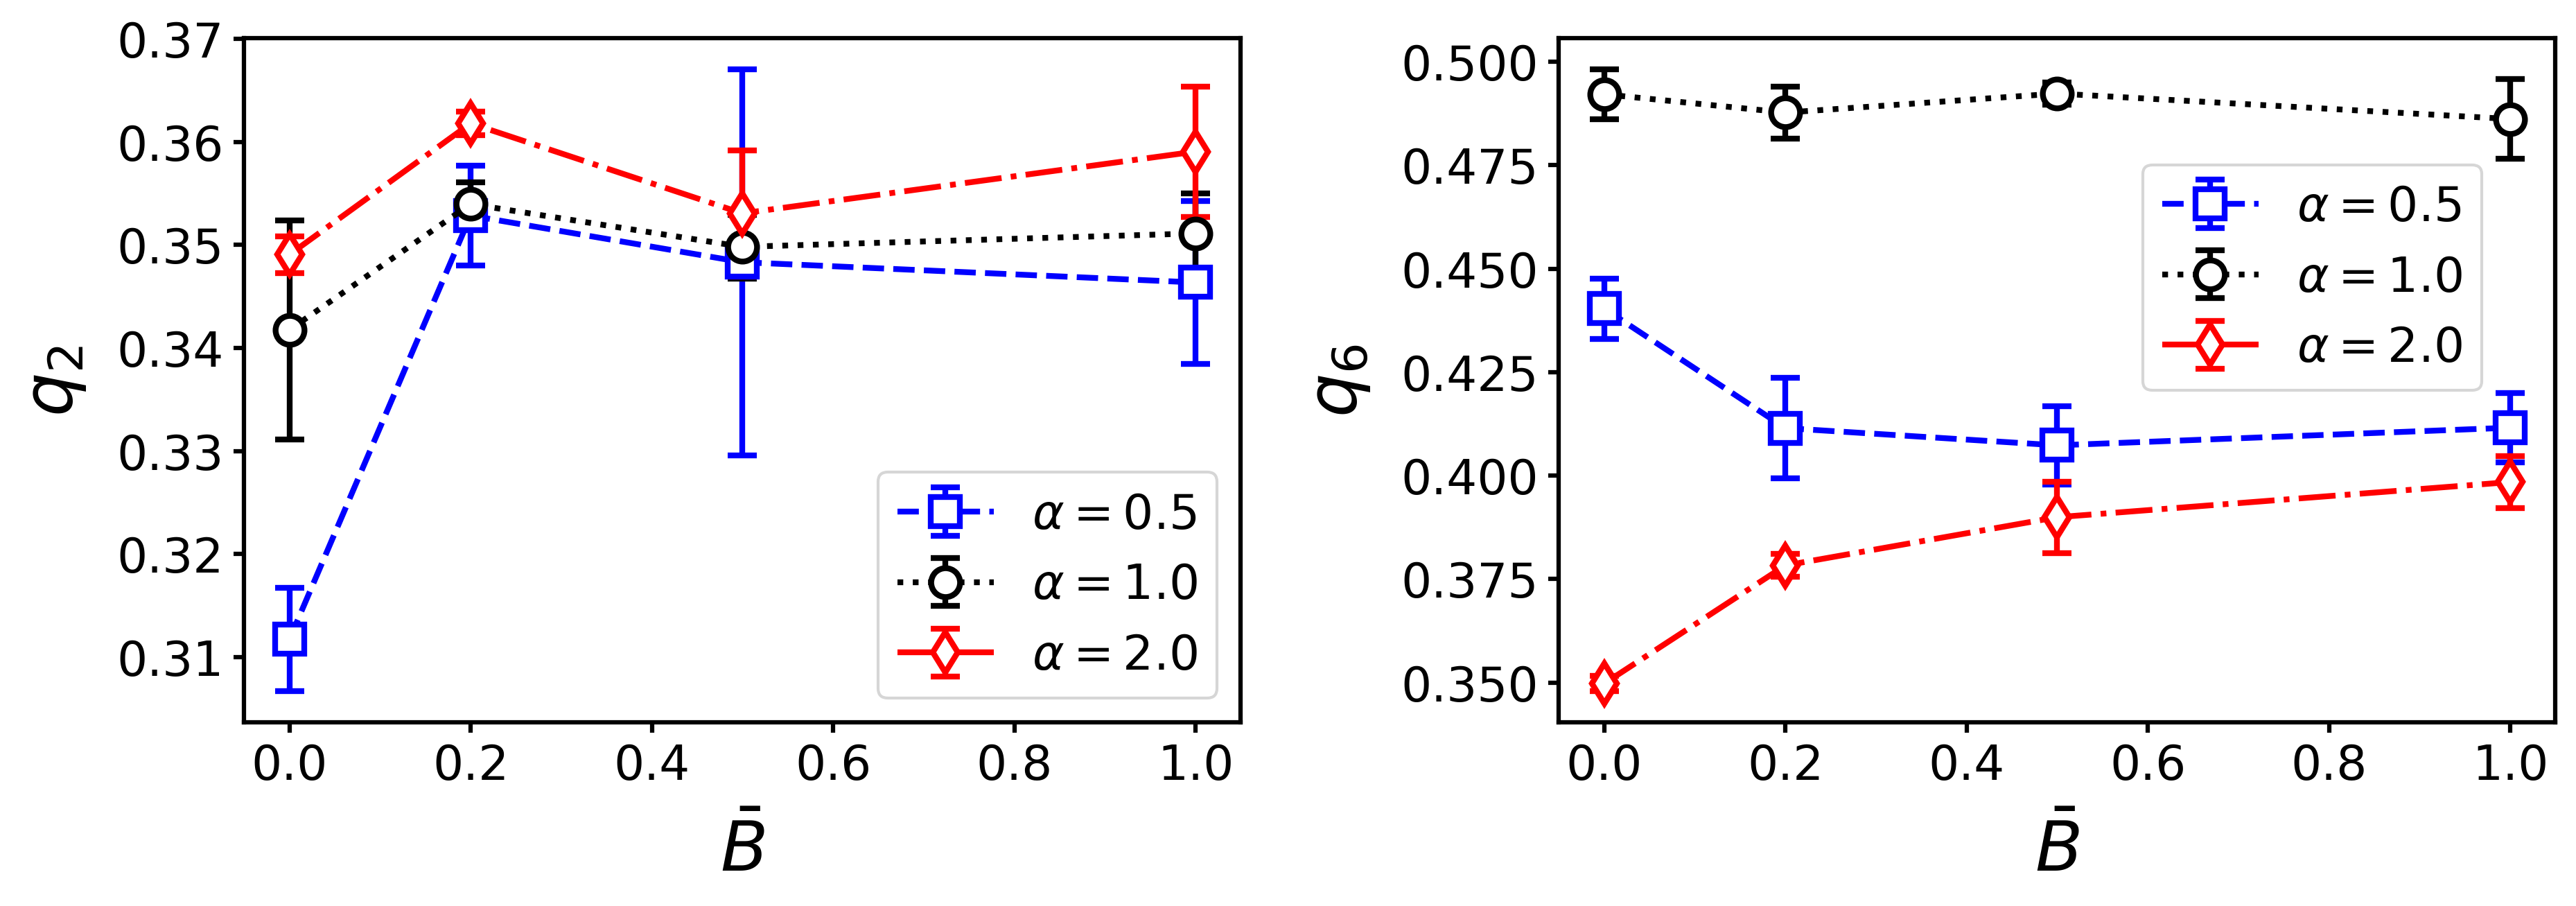
\includegraphics[scale=0.45]{../figures/results/paper1_5/steinhardt_field.png}%
\caption{Dependence of the Steinhardt order parameter $q_2$ and $q_4$ on the magnetic field $\bar{B}$. The order parameters were computed for the final 
         bijel microstructure after $10^5$ simulation time steps. Errorbars indicate the standard deviation taken over three independent simulation runs.
\label{fig:steinhardt_field}}%
\end{figure}

Figure~\ref{fig:steinhardt_field} presents the variation of the bond orientational order parameters \(q_2\) and \(q_6\) with magnetic field strength for fully arrested bijel structures at \(10^5\) 
timesteps. The consistently finite values of \(q_2\) across all field strengths indicate that the interfacial particle arrangements lack long-range crystalline order, irrespective of whether a magnetic 
field is applied. Notably, \(q_2\) remains largely unaffected by the strength of the applied field. In contrast, \(q_6\), which reflects the degree of six-fold orientational symmetry, varies with both 
particle shape and magnetic field. For spherical particles, \(q_6\) reaches the highest values, while for ellipsoidal particles, the magnitude of \(q_6\) is generally reduced. In the case of oblate 
(disk-like) ellipsoids, \(q_6\) decreases as the magnetic field increases, whereas for prolate (rod-like) ellipsoids, \(q_6\) grows with increasing field strength, though it remains lower than that 
observed for oblate particles. These results suggest that magnetic alignment promotes six-fold ordering in the interfacial monolayer, with the extent of ordering modulated by particle aspect ratio. 
For prolate particles, the elongated shape imposes geometric constraints that suppress perfect six-fold symmetry. Meanwhile, the reduced \(q_6\) for oblate particles under strong fields may be attributed 
to out-of-plane tilting or stacking effects relative to the interface \cite{dabat_mesoscale_2018}. Overall, while the interfacial layers exhibit some degree of six-fold order in two dimensions, the 
non-zero \(q_2\) values confirm that the particle arrangement remains amorphous in three dimensions due to interfacial curvature. This motivates further exploration of how the trends in \(q_6\) with 
field strength relate to changes in the mean and Gaussian curvature of the interface.

\subsection{Curvature of the interface}

Interfacial curvature provides geometric descriptors that complement other measures of bijel morphology and are directly relevant to understanding transport properties in the resulting porous structure.
\cite{reeves_quantitative_2016} The local principal curvatures \(\kappa_1\) and \(\kappa_2\) are obtained as the inverse of the radii of curvature, \(R_1\) and \(R_2\) and are used to calculate
the area averaged mean $H$ and Gaussian $K$ curvatures.

\begin{align}
\langle H \rangle &= \frac{1}{A}\int_A \frac{\kappa_1+\kappa_2}{2} \mathrm{d}A , \\
\langle K \rangle &= \frac{1}{A}\int_A \kappa_1\kappa_2 \mathrm{d}A .
\end{align} 

To compute curvature, we begin by calculating 
the order parameter field \(\phi(\vec{x}) = \rho^{b}(\vec{x}) - \rho^{r}(\vec{x})\), defined as the local density difference between the two fluid components at each lattice site. Since the presence 
of colloidal particles creates voids in the density field, we apply a particle-filling procedure similar to that used in dynamic simulations to fill uncovered grid points. This step iteratively fills 
the lattice nodes occupied by particles using local averaging from surrounding fluid nodes, thereby reconstructing a continuous order parameter field that more accurately represents the interface geometry.
From the completed \(\phi\) field, we extract the bijel interface as the \(\phi = 0\) isosurface using the marching cubes algorithm implemented in the \texttt{scikit-image} library \cite{van2014scikit}. 
We then compute the mean and Gaussian curvatures of the interface using the \texttt{PyVista} package \cite{sullivan2019pyvista}. and are used to compute the Gaussian curvature \(K = \kappa_1 \kappa_2\) and mean curvature \(H = \frac{1}{2}(\kappa_1 + \kappa_2)\) at each mesh vertex.


\begin{figure}
    \centering
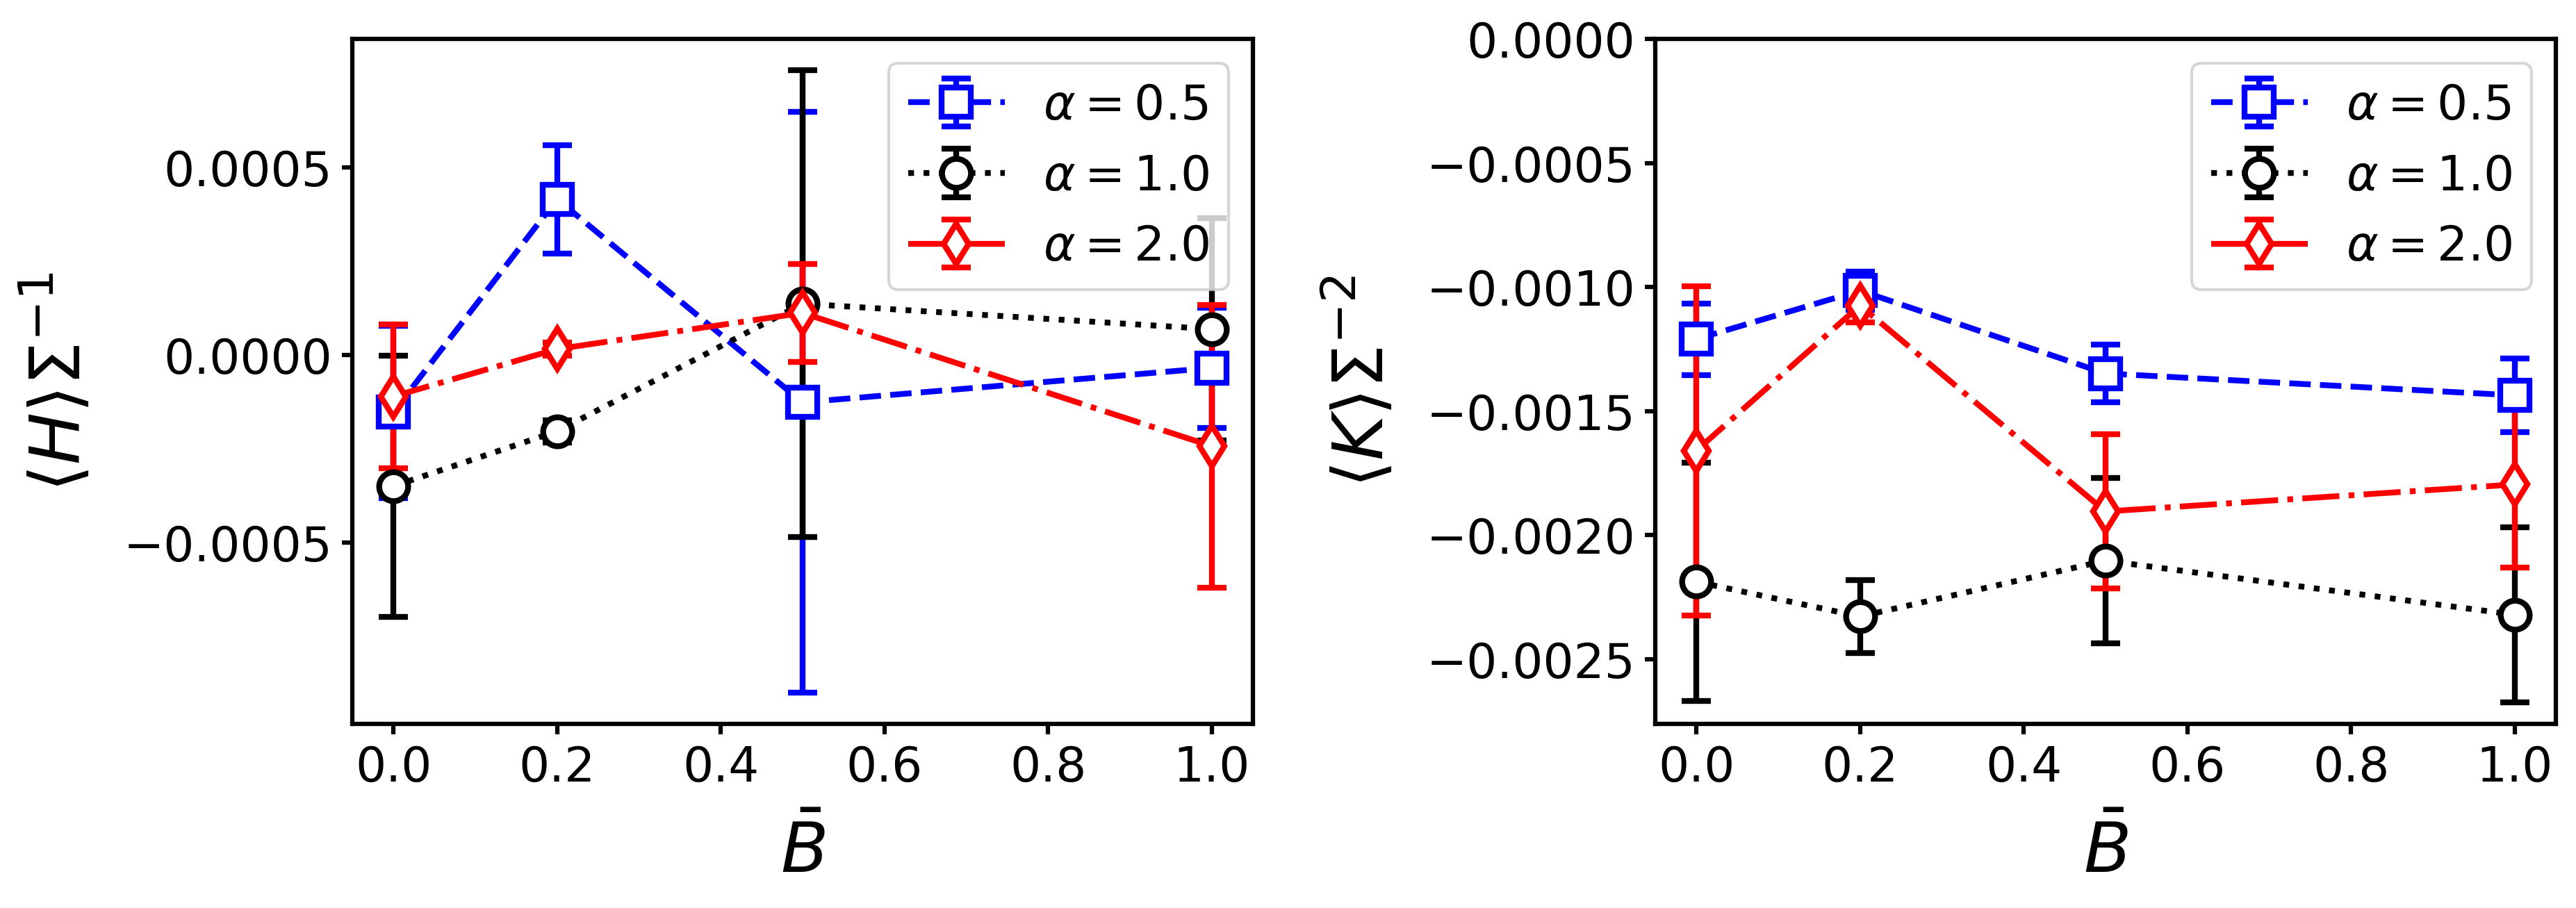
\includegraphics[scale=0.5]{../figures/results/paper1_5/curvature_field.png}%
\caption{Plot of the area averaged mean $\langle H \rangle \Sigma^{-1}$ and Gaussian $\langle K \rangle \Sigma^{-2}$ curvature in the left and right 
         respectively. Each plot contains the $\langle H \rangle \Sigma^{-1}$ and $\langle K \rangle \Sigma^{-1}$ at the final timestep averaged across 
         3 runs for particles with $\alpha = 0.5, 1, 2$. We observe that the mean curvature does not demonstrate any trends, while the Gaussian curvature 
         shows a reduction as the magnetic field strength is increased for ellipsoidal particles.}
\label{fig:curvature_field}%
\end{figure}

Figure~\ref{fig:curvature_field} shows the dependence of the area-normalized mean and Gaussian curvature,\(\langle H \Sigma^{-1} \rangle\) and \(\langle K \Sigma^{-2} \rangle\) respectively, on the 
applied magnetic field strength. As expected for systems with equal fluid volume fractions and neutrally wetting particles, the mean curvature remains close to zero across all field strengths and shows 
no significant field dependence, reflecting the absence of a preferred direction for interfacial bending \cite{jinnai_interfacial_2001}. In contrast, the Gaussian curvature exhibits a clear trend for 
ellipsoidal particles, becoming increasingly negative with higher magnetic field strength. This indicates that the interface adopts a more pronounced saddle-like geometry as the field strengthens.
Previous work has shown that bijels formed with smaller stabilizing particles, such as nanoparticles, exhibit more negative Gaussian curvature due to their enhanced ability to conform to curved interfacial 
geometries \cite{reeves_quantitative_2016}. This behavior is attributed to their smaller cross-sectional area, which introduces minimal disruption to the hyperbolic character of the interface. Consistent 
with these findings, our zero-field results show that ellipsoidal particles produce less negative Gaussian curvature than spheres. Specifically, the oblate and prolate particles used here have approximately 
60\% and 30\% larger cross-sectional areas, respectively, compared to spheres of the same volume. However, under increasing magnetic field strength, these anisotropic particles align with the field direction, 
effectively reducing their projected area at the interface. This reorientation enables the interface to adopt more negatively curved geometries, explaining the observed decrease in 
\(\langle K \Sigma^{-2} \rangle\) with field strength. These curvature changes suggest corresponding shifts in the topology of the bijel structure, motivating a closer examination of its topological features.


\subsection{Topology of the emulsion microstructure}

Domain size is one of the most widely used metrics for characterizing coarsening in emulsions. Common approaches to determine domain size include calculating the moments or identifying peaks in the structure 
factor, which are often used to detect dynamic scaling regimes \cite{kendon_inertial_2001}. However, these definitions do not always yield an accurate representation of the true domain dimensions 
\cite{karthikeyan_formation_2024}, and domain size alone does not fully capture morphological variations in bijels under different processing conditions \cite{reeves_quantitative_2016}. The Gauss-Bonet
theorem connects the curvature of a surface to its topology through parameters such as the genus($g$) which can be thought of as the number of holes in a surface. Spheres and torii have a genus of 0 and 1 respectively. 
In this context, we also calculate the number of handles($h$) defined as channels through the volume and voids($v$) which characterize the number of disconnected cavities or loops. The relation between genus \(g\), 
number of handles \(h\), and number of voids \(v\) is thus expressed by \cite{chan_channel_2012}

\begin{equation}
g = h - v .
\end{equation} 

The genus is related to the Euler-Poincar\'e characteristic \(\chi\) of the surface, i.e., 

\begin{equation}\label{eq:genus}
g = 1 - \frac{\chi}{2} .
\end{equation} 

To compute the Euler-Poincaré characteristic, we used the \texttt{skimage.measure.euler\_number} function from the scikit-image library. In this implementation, the Euler characteristic is defined as the 
number of objects plus the number of holes minus the number of loops, effectively incorporating the factor of 1/2 in Eq.~\ref{eq:genus} into the returned value. As a result, the genus \(g\) was determined 
by subtracting the Euler characteristic from the total number of connected objects. The number of voids was calculated using \texttt{skimage.measure.label}, also from scikit-image, by identifying and 
excluding all regions connected to the boundary of the simulation volume. The number of handles was then obtained by applying Eq.~\ref{eq:genus}.

\begin{figure}
    \centering
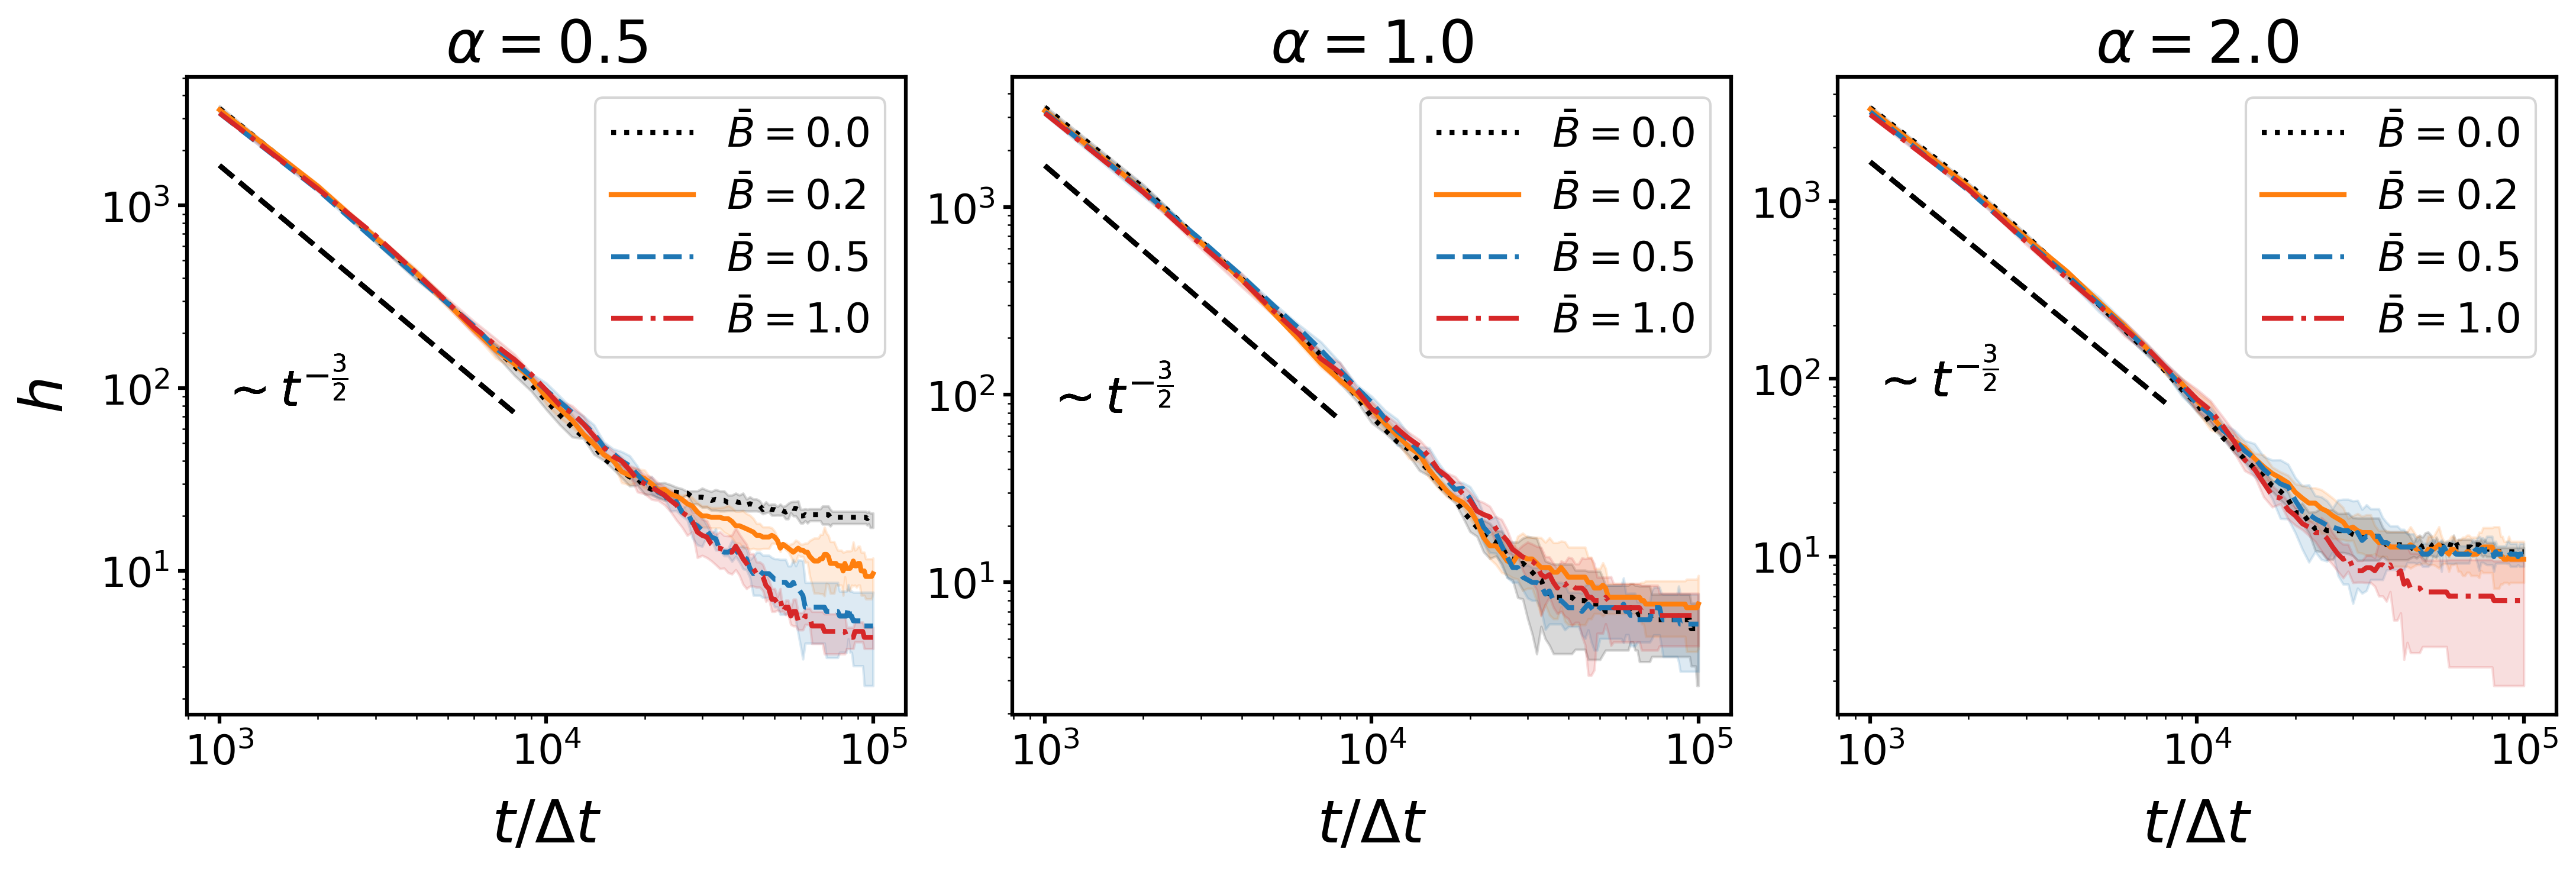
\includegraphics[scale=0.45]{../figures/results/paper1_5/handles_time.png}%
\caption{Time dependence of the number of channels for different particle shapes $\alpha$ and at different magnetic field strength $\bar{B}$. 
         The bands around the lines indicate the standard deviation taken over three independent simulation results. The number of channels roughly 
         follows a power law behavior $\sim t^{-3/2}$ which suggests that it is inversely proportional to the characteristic domain size $L \sim t^{3/2}$.
\label{fig:handles_time}}%
\end{figure}

The temporal evolution of the number of handles—interpretable as the number of continuous channels through the volume—is presented in Fig.~\ref{fig:handles_time}. This measure provides insight 
into coarsening dynamics, particularly the occurrence of coalescence and pinch-off events. Across all simulations, regardless of particle shape or magnetic field strength, the number of channels 
decreases over time following a similar trend. During the coarsening phase, this decrease closely follows a power law relationship \(h \sim t^{-2/3}\), which is consistent with the known scaling 
law for the domain size \(L \sim t^{2/3}\). This inverse relationship suggests that the number of channels is proportional to the inverse of the characteristic domain size. 
Neither particle anisotropy nor magnetic field strength significantly alters this dynamic scaling behavior during the early stages of coarsening. However, once jamming begins, the reduction in the 
number of channels slows down, though it does not stop entirely. This behavior aligns with earlier findings by Harting and collaborators \cite{gunther_timescales_2014}, which identified multiple 
timescales governing bijel formation. Additionally, we observe that higher magnetic field strengths tend to delay the onset of jamming, consistent with previous observations of reduced coarsening 
rates under such conditions \cite{karthikeyan_formation_2024}.
Following jamming, the final number of channels varies with particle shape and magnetic field strength, likely reflecting the specific domain morphology present at the onset of structural arrest. 
Some regions may already be immobilized while others remain dynamic, contributing to the slow, continued reduction in channel number. Nevertheless, our results do not reveal a clear or systematic 
dependence of the final channel count on particle anisotropy or field strength.

%\TODO{need some comments on coarsening kinetics here and literature references, e.g., comparing to number of droplets over time}

To characterize topological changes in the bijel structure, we compute the channel size distribution (CSD) following the method developed by Chan and Thornton \cite{chan_channel_2012}. This approach begins 
with the construction of a signed distance field from the order parameter \(\phi\), which is reinitialized using the level set algorithm described by Sussman et al.~\cite{sussman_level_1994, chan_channel_2012}. 
The resulting distance transform is smoothed using a boxcar-averaging stencil with periodic boundary conditions to reduce numerical artifacts arising from grid discretization \cite{chan_channel_2012}. 
From the smoothed distance field, a series of isosurfaces are extracted at normalized distances \(\bar{r} = r \cdot \Sigma\), where \(\Sigma\) is the specific interfacial area. The number of handles is computed 
for each of these isodistance surfaces. A decrease in the number of handles with increasing distance from the interface reflects the pinch-off of channels, providing insight into the evolving connectivity of the 
microstructure. The channel size distribution is then obtained from the negative derivative of the handle count with respect to \(\bar{r}\), yielding a statistical measure of channel sizes as a function of 
distance from the interface.

\begin{equation}
f(r) = - \frac{d h(r)}{dr} .
\end{equation}

\begin{figure}
    \centering
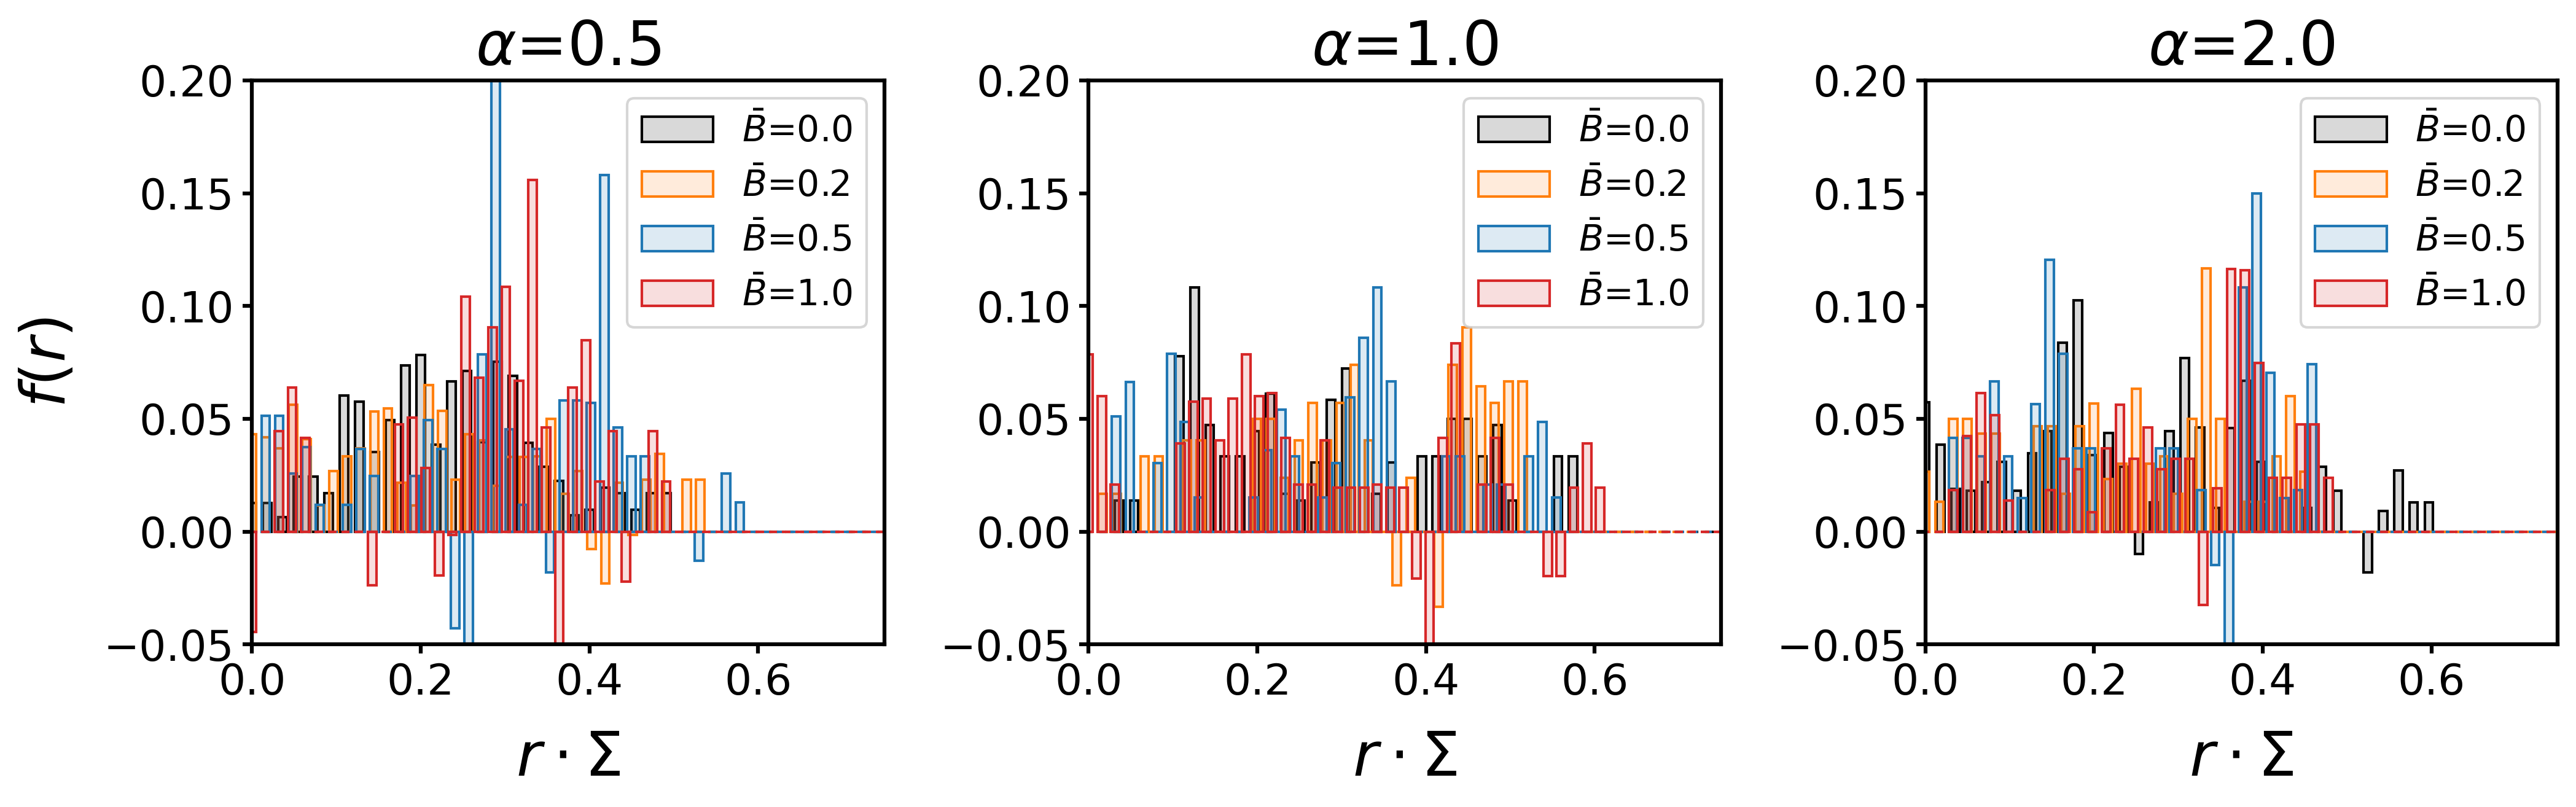
\includegraphics[scale = 0.4]{../figures/results/paper1_5/CSD.png}%
\caption{Channel size distribution (CSD) in bijels stabilized by oblate ($\alpha=0.5$), spherical ($\alpha=1.0$), and prolate ($\alpha=2.0$) particles. 
         The channel size distribution was obtained as the negative derivative of the number of handles in isodistance structures of the Euclidean distance 
         transform of the order parameter field. The negative values are due to numerical artifacts when calculating the number of handles as a function of 
         isodistance from the interface.}
\label{fig:CSD}%
\end{figure}

Figure~\ref{fig:CSD} presents the channel size distribution (CSD) for bijels formed with three different particle shapes under varying magnetic field strengths. Minor negative values appear in 
the distribution due to numerical artifacts associated with computing the number of handles as a function of distance from the interface. Overall, we do not observe any consistent or systematic 
trends related to particle shape or field strength. The channel sizes span a broad range, extending up to approximately \(0.6 \cdot \Sigma^{-1}\), which corresponds to about 20\% of the total system 
size. This wide distribution reflects the structural complexity of bijel morphologies, which include both broad channels and narrow regions where opposing interfaces are separated by distances 
comparable to the particle size. Although previous results indicated anisotropic domain sizes, suggesting the possibility of a bimodal channel distribution, such a feature is not evident in the 
present data. It is possible that a larger simulation domain would be required to resolve such effects more clearly, which could be explored in future work.

\begin{figure}
\centering
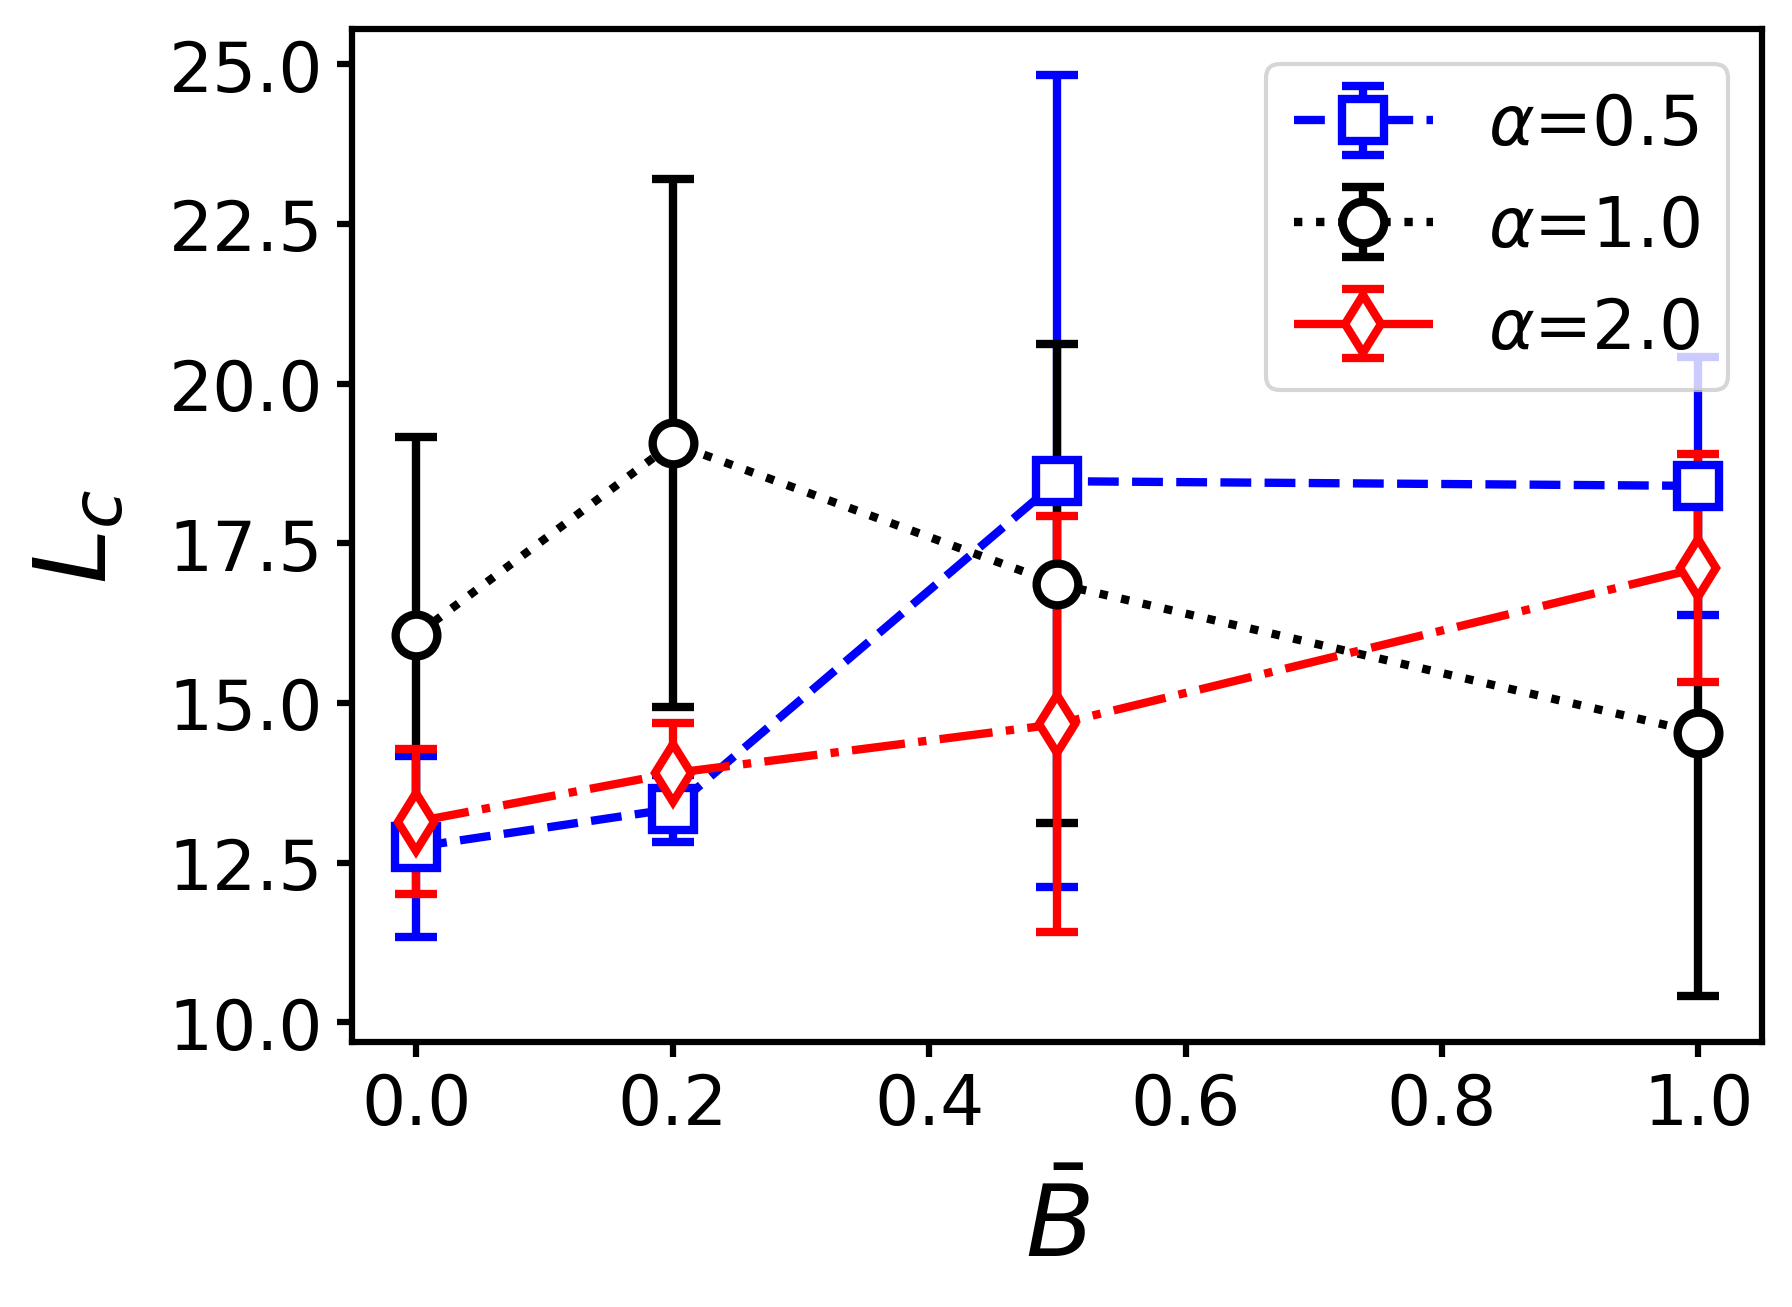
\includegraphics[scale = 0.6]{../figures/results/paper1_5/channel_size_field.png}%
\caption{Average channel size $L_c$ for different particle shapes $\alpha$ and at different magnetic field strength $\bar{B}$. The average channel size was calculated from the channel size distribution shown in Fig.~\ref{fig:CSD}. Errorbars indicate the standard deviation taken over three independent simulation runs.
\label{fig:channel_size_field}}%
\end{figure}

To relate the channel size distribution (CSD) to previous estimates of the characteristic domain size, we calculated the average channel size \(L_c\), shown in Fig.~\ref{fig:channel_size_field}. For 
systems stabilized by spherical particles, we observe relatively large error bars, representing the standard deviation across three independent simulations. This variability is likely due to the 
sensitivity of the final microstructure to the initial particle arrangement, which can influence the timing of jamming and the pathways available for coarsening—as reflected in the time evolution of 
the number of channels. In contrast, for anisotropic particles, the average channel size increases with magnetic field strength. This trend, along with the overall scale of \(L_c\), is in good agreement 
with previous domain size measurements based on structure factor moments (see Fig. 4 in Ref.~\citenum{karthikeyan_formation_2024}). Thus, identifying channel sizes through topological analysis of 
isodistance surfaces offers an alternative and complementary approach to quantifying domain size in bicontinuous emulsions. Moreover, this method reveals additional insights into the coarsening dynamics 
that are not captured by traditional geometric or structural metrics.

\section{Conclusion}
% \section[Conclusion]{Conclusions\protect\footnote{This section is based on work submited to the American Institude of Physics, Physics of Fluids journal.
% It is reproduced from submission number \#POF25-AR-DSFD2024-03180, with the permission of AIP Publishing.}}


We analyzed the structural properties of bijels stabilized by magnetic ellipsoidal particles using data from Lattice Boltzmann–Molecular Dynamics simulations of binary mixtures containing oblate, 
spherical, and prolate magnetic particles across varying magnetic field strengths. Structural characterization included bond orientational order via Steinhardt parameters, interfacial mean and 
Gaussian curvature, and topological features of the emulsion morphology. In the jammed state, particle layers showed evidence of six-fold ordering but lacked crystalline symmetry in 3D due to 
interfacial curvature. We also found that anisotropic particles induce greater Gaussian curvature than spheres, while increasing magnetic field strength reduces Gaussian curvature—suggesting that 
magnetic alignment enhances the hyperbolic nature of interfaces, promoting more robust bijel formation with anisotropic particles.

To track coarsening, we quantified topological evolution through the number of handles, which reflects the count of channels in the bicontinuous structure. This number decreases over time following a 
power-law trend inversely proportional to domain size. The decay rate slows after jamming, consistent with prior findings \cite{gunther_timescales_2014, karthikeyan_formation_2024}. We further 
extracted channel size distributions (CSDs) from isodistance surfaces of the level set reinitialization \cite{chan_channel_2012}, revealing a broad range of channel sizes without systematic 
changes across magnetic field strengths. However, the average channel size from the CSD agrees with previous domain size measurements.

Our results bridge multiple aspects of bijel morphology: interfacial particle packing connects to local curvature, while global topological features relate to coarsening events such as domain 
coalescence and channel pinch-off. This study extends previous curvature analyses by Reeves et al.~\cite{reeves_quantitative_2016} and CSD measurements in Cahn-Hilliard systems by Chan and 
Thornton \cite{chan_channel_2012}, offering a more detailed view than conventional global metrics like domain size. These structural descriptors are also relevant for applications: interfacial 
particle order correlates with yield stress in emulsions \cite{besseling_three-dimensional_2007, schall_structural_2007, madivala_exploiting_2009, vagberg_glassiness_2011, kaganyuk_shear-induced_2020}, 
and interface curvature affects cell adhesion and reaction kinetics in energy systems \cite{xiong_porosity_2024, shojaei_minimal_2022}.
Understanding how these properties depend on formulation and processing conditions is key for bijel design. By analyzing independent simulations with varied initial conditions, we also captured 
statistical variation in features like channel size and its distribution. These insights lay the groundwork for systematic tuning of bijel fabrication. In particular, magnetic ellipsoidal particles 
offer promising avenues for controlled modulation of interfacial structure and domain morphology.